\section{Model}
\label{sec:model}

\setlength{\tabcolsep}{2pt}
\begin{figure*}
\begin{center}
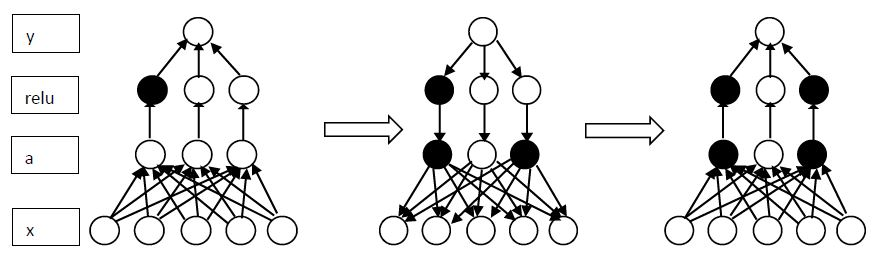
\includegraphics[width=0.95\linewidth]{figs/model/iteration}
% \vspace{-10pt}
\caption{Illustration of our feedback model and its inference process. At the first iteration, the model performs as a feedforward neural net. Then given the top signal neuron, the hidden layers update their gates to maximize the confidence for the top neuron. This process continues until convergence.}
\label{fig:visual_compare}
% \vspace{-30pt}
\end{center}
\end{figure*}

\subsection{Convolutional Neural Networks}

\subsection{Infering the Hidden Neurons, the Discriminative Framework}

\subsection{Class Model Visualization}

\textbf{Relationship to Oxford and Deconv}

\subsection{Object Localization}

\textbf{Relationship to Oxford and Deconv}
